% !TeX root=tukedip.tex
% !TeX encoding = UTF-8
% !TeX spellcheck = sk_SK
\section{Metódy riadenia v multi-robotických systémoch}
V organizácii a správe systémov s niekoľkými mobilnými robotmi v súčasnosti existuje veľa rôznych prístupov. Nedá sa povedať, že existujú správne alebo nesprávne prístupy, každý zo systémov má svoje výhody aj nevýhody. Rozhodnutie o použití systému sa prijíma na základe konkrétnej úlohy projektu.
V tejto časti sa pozrieme na rôzne metódy riadenia a organizácie multi-robotických systémov, ako aj na ich výhody a nevýhody.

\subsection{Multi-robotické systémy}

Systémy viacerých robotov sú dobré z mnohých ďalších dôvodov. Podľa Aparicio a Lima \citep{aparicio} systémy s viacerými robotmi  ponúkajú robustnosť a prispôsobivosť, aké sa v systémoch s jedným robotom nenachádzajú. Ak je jeden agent v systéme poškodený alebo nefunguje správne, je možné úlohu dokončiť so zvyšnými agentmi. Túto myšlienku možno uplatniť aj pri údržbe. Agenti môžu byť obsluhovaní po jednom, čo vedie k skutočnosti, že systém nie je nečinný, ak sú ostatní roboti schopní pokračovať v plnení úlohy bez prítomnosti ich partnera. Viaceré roboty navyše dokážu pokryť veľkú oblasť a môžu sa špecializovať na menšie úlohy, ktoré postupujú k splneniu väčšej úlohy \citep{aparicio}. Preto je pravdepodobnejšie, že systémy s viacerými robotmi budú spoľahlivo vykonávať veľké a zložité úlohy. Napriek mnohým výhodám systémov viacerých robotov je potrebné vyriešiť niekoľko nevýhod. Najskôr je komunikácia medzi agentmi v systéme výpočtovo zložitá. Podľa Coesa, Nurbakhsh a Sikar %\citep{koes} 
, keď sa systémy s viacerými robotmi rozhodnú, musia brať do úvahy čas potrebný na cestu na konkrétne miesto, čas čakania na príchod ďalších robotov a čas na dokončenie úlohy. V dôsledku toho sú riadiace algoritmy veľmi zložité, pretože systém sa implementuje ťažšie, ak na konkrétnom probléme pracuje viac agentov. Rádiová komunikácia dodáva systému ďalšiu vrstvu zložitosti, pretože si vyžaduje použitie prenosových obvodov a komunikačných protokolov. Preto, aj keď môže byť systém s viacerými robotmi efektívnejší, tento však vyžaduje väčšiu zložitosť než systém s jedným robotom. 

\subsection{Praktické využitie multi-robotických systémov}

Počas výskumu boli objavené aplikácie, ktoré priamo súvisia s mojím projektom. V jednom konkrétnom príklade boli na
premiestnenie nábytku na konkrétne miesta použité dva veľké roboty. V praktickejšom príklade je možné použiť roboty na
presun ťažkých materiálov na stavenisku. Je pravdepodobné, že roboty s takouto úlohou veľmi pomôžu a môžu zvýšiť
efektivitu, ale roboty sú zvyčajne príliš drahé na to, aby boli finančné prospešné.
\vspace{3mm}

\justifying
\noindent 
Jednou z možností v súčasnosti je použitie koordinovaných robotov na skúmanie oblastí, ktoré by mohli byť pre
človeka nebezpečné. Tieto roboty môžu autonómne zvyšovať bezpečnosť alebo vytvárať nebezpečné oblasti. Napríklad oblasť
plná mín môže byť vhodná pre robotov vybavených senzormi určenými na detekciu mín. Potom, čo v mínovom poli, bude robot schopný rozpoznať mínu bez účasti ľudí. nájdení bane môže robot oznámiť polohu míny ďalším robotom.
Ostatní roboti pomocou koordinačných algoritmov a pozičných senzorov budú môcť k míne pristúpiť a pomôcť ju rozobrať
alebo označiť. Roboti sa môžu navzájom rozprávať alebo môžu používať hlavného robota, ktorý dáva každému z nich smer
\citep{mclurkin}. Projekt, ktorý je rovnako jednoduchý ako koordinované tlačenie škatúľ robotom, slúži ako východiskový bod pre
zložitejší a užitočnejší systém, ako sú napríklad robotické vyhľadávače mín.

\subsection{Ovládanie multi-robotických systémov}
Ovládanie systému s viacerými robotmi je vo všeobecnosti náročným problémom. K tejto otázke existujú dva prístupy:
centralizovane riadenie a decentralizovane riadenie \citep{kexu}.

\subsubsection{Centralizovaný systém}
V centralizovanom systéme s niekoľkými robotmi sa ukladajú globálne informácie o stave celého systému. Systém
zhromažďuje informácie o všetkých robotoch a sleduje ich polohu v prostredí. Na základe informácií získaných od robotov
dokáže zostaviť mapu. Tento systém je buď na stacionárnom hostiteľovi, alebo v jednom robote, ktorý zjavne funguje ako
hlavný. Potom majster zorganizuje tím robotov, aby dosiahli spoločný cieľ a naplánuje úlohy pre jednotlivých členov tímu
a dohliada na celý proces.
Táto architektúra sa dá ľahko navrhnúť, ale nie je odolná voči výpadkom komunikácie a nepredvídateľným situáciám.
Centralizované riadenie je zvyčajne vhodné pre obmedzený počet robotov, ktorí pracujú v známom a nemennom prostredí.

\subsubsection{Decentralizovaný systém}
Naproti tomu decentralizované systémy nezahŕňajú žiadneho riaditeľa, ktorý má úplné informácie o stave systému a riadi
celý proces. Naopak, každý robot je autonómna jednotka, ktorá koná v súlade so stavom svojho prostredia. Robot si je
samozrejme vedomý prítomnosti ďalších robotov a môže s nimi komunikovať na miestnej úrovni. Komplexné skupinové
správanie vyplýva z interakcií medzi robotmi a prostredím. Táto architektúra je veľmi robustná, môže dobre fungovať v
nepriateľskom prostredí a je škálovateľná, potenciálne obrovské množstvo homogénnych robotov môžu spolupracovať na
dosiahnutí spoločného cieľa.

\subsection{Problématika riadenia}
Problém s riadením v navigácii mobilných robotov sa rieši dvoma spôsobmi: deliberatívnym a reaktívnym riadením (Obrázok 2 –
1).

\begin{figure}[ht!]
    \centering
    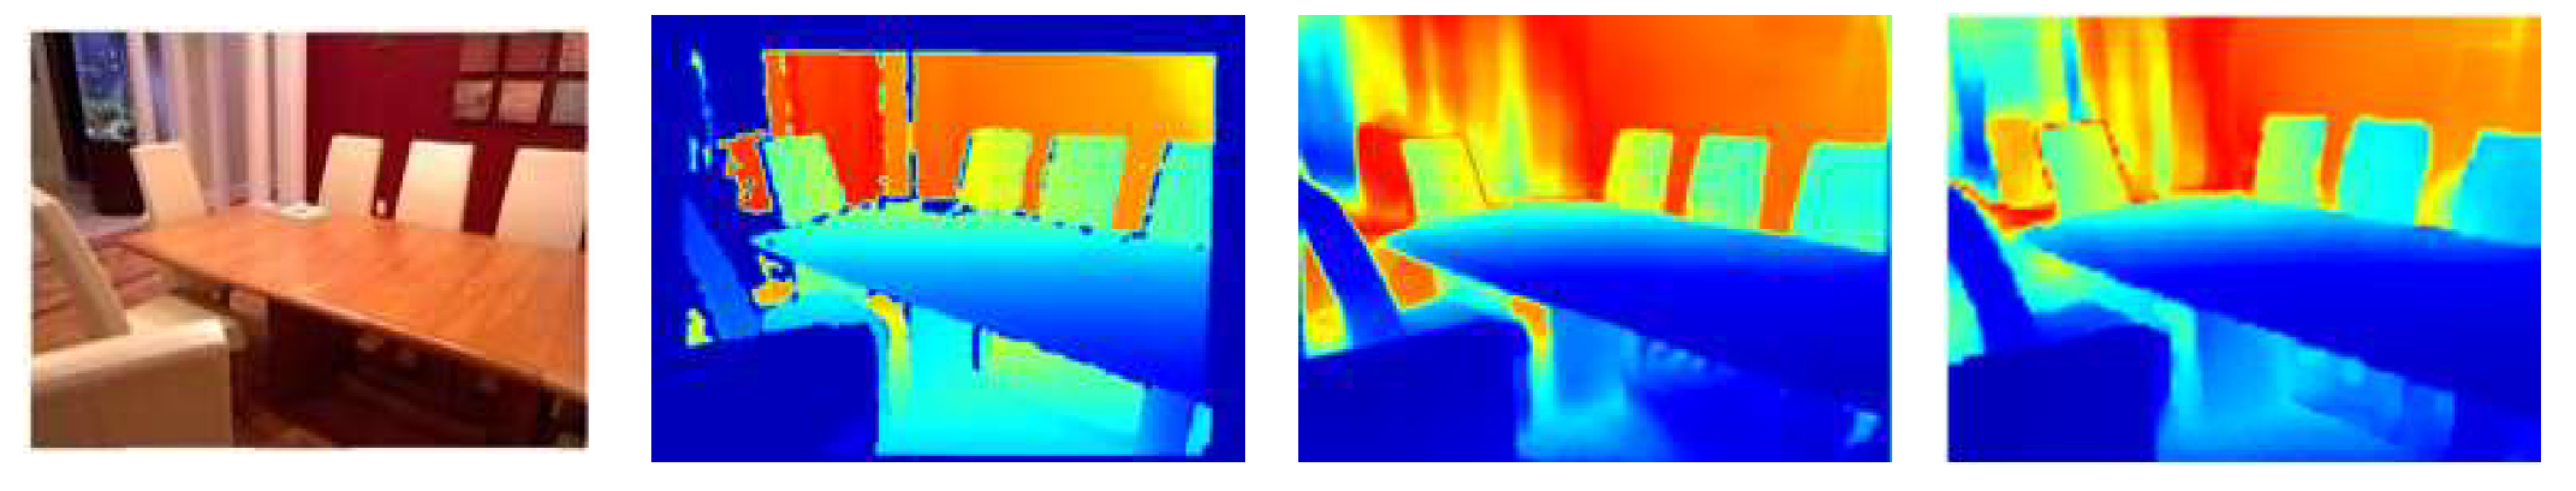
\includegraphics[width=.85\textwidth,angle=0]{figure 2-1.pdf}
    \caption{Stratégie riadenia navigácie v formácií.}
    \label{o:3}
\end{figure}

\subsubsection{Deliberatívne riadenie}
Prístup založený na plánovaní pohybu a trajektórie pohybu vyžaduje predbežné znalosti prostredia na plánovanie pohybov
robotov \citep{vascak}. Tento prístup využíva formalizmy ako Voronoiove diagramy alebo umelé potenciálne funkcie \citep{rimon},
pričom zohľadňuje všeobecné poznatky o životnom prostredí. Plánovanie pohybu je všeobecne optimálne z hľadiska
efektívnosti / reaktivity. V skutočnosti sa pre mierku veľmi veľkého počtu robotov nemodifikujú dobre kvôli výpočtovej
zložitosti. Vďaka predchádzajúcim znalostiam prostredia však roboti svoju misiu zvyčajne úspešne dokončia dobrým
výkonom.

\subsubsection{Reaktívne riadenie}
Pri reaktívnej metóde, roboty konajú iba podľa informácií svojich miestnych senzorov bez akýchkoľvek
ďalších všeobecných znalostí. Techniky založené na správaní sú vynikajúcou ilustráciou reaktívnej kontroly.
Globálna úloha robota je v skutočnosti rozdelená na súbor čiastkových úloh (vzorce správania).
Podľa informácií o senzore je stratégia riadenia použitá na robota založená na jednom zvolenom vzorci správania 
alebo je zlúčením niekoľkých vážených modelov. Keď aplikácia vyžaduje, aby roboty fungovali v reálnom čase (napríklad v nebezpečných
prostrediach), je zrejmé, že reaktívne metódy sa stávajú oveľa zaujímavejšími ako plánovanie pohybu \citep{vascak}.

\paragraph{Hierarchická stratégia.}
Pri prvom prístupe sa jeden alebo viac robotov považuje za vedúcich a iné roboti sú ďalší. Vedúci typicky sleduje danú
trajektóriu, zatiaľ čo nasledovníci sledujú jej transformované súradnice. Tento prístup sa dá ľahko sledovať.
Je však zaznamenané, že problém s hlavným robotom spôsobí zastavenie celého systému. V prístupe distribuovaného správania, 
neexistuje medzi robotmi hierarchia. Každý má svoje vlastné vnímanie a kontrolu a porucha robota nevedie k zlyhaniu
skupiny \citep{vascak}.

\paragraph{Stratégia správania.}
Stratégia založená na správaní znamená, že každý robot má súbor správania (základné úlohy), ktoré musia byť vykonané.
Výsledné skupinové správanie vyplýva zo základnej lokálnej interakcie bez explicitného vzoru celkového kooperatívneho
správania. Tento prístup však bol kritizovaný za to, ako volí riadenie pre každého robota. Podľa informácií o vnímaní
riadiaci systém v skutočnosti prepína medzi správaním (napríklad konkurenčný prístup) alebo kombinuje niekoľko
ovládačov (napríklad motorický obvod). To prirodzene sťažuje štúdium udržateľnosti stratégie globálneho riadenia \citep{ogren}.

\paragraph{Stratégia virtuálnej štruktúry.}
Virtuálna štruktúra (tretí prístup) považuje vzdelávanie za jediné virtuálne telo. Tvar posledného menovaného je
požadovaný tvar formácie a jeho pohyb sa prevedie na požadovaný pohyb každého vozidla. Virtuálna štruktúra
bola implementovaná v niekoľkých dielach s využitím potenciálnych metód poľa: teda všetky prvky formácie
sledujú pridelené uzly, ktoré prechádzajú do požadovanej konfigurácie. Na rozdiel od plánovania
pohybu využívajú potenciálne funkcie použité pri prístupe k virtuálnej štruktúre iba okamžité a lokálne vnímanie
robotov. Nedostatočné využitie potenciálnych prvkov pre tento druhý prístup zodpovedá zvyšujúcej sa zložitosti riadenia
tvaru flotily v dynamickom prostredí. To v skutočnosti znamená, že robot je vystavený často sa meniacemu počtu /
amplitúde síl, čo vedie k ďalším lokálnym minimám, fluktuáciám atď. Preto je v tomto prípade veľmi ťažké preukázať
spoľahlivosť a stabilitu navigácie \citep{ogren}, \citep{vascak}.



\subsection{Multi-robotické systémy podľa typovosti}
Skupinu robotov definujeme ako homogénnu, ak sú možnosti jednotlivých robotov rovnaké a inak skupina je heterogénna. Heterogenita
vo všeobecnosti prináša zložitosť, pretože alokácia úloh sa stáva zložitejšou a agenti majú väčšiu potrebu modelovať
ďalších robotov v skupine. Existuje koncept pokrytia úlohy, ktorý meria schopnosť daného člena tímu dosiahnuť danú
úlohu. Tento parameter predstavuje index dopytu po spolupráci: keď je pokrytie úloh vysoké, úlohy je možné splniť bez
väčšej spolupráce, ale inak je spolupráca nevyhnutná. Pokrytie úlohy je maximálne v homogénnych skupinách a klesá, keď
sú skupiny čoraz viac heterogénne (t. j. v krajnom prípade môže danú úlohu vykonať iba jeden agent v skupine).
V literatúre v súčasnosti prevládajú diela, ktoré predpokladajú homogénne skupiny robotov. Niektoré pozoruhodné
architektúry však dokážu zvládnuť heterogenitu, napr. ACTRESS a ALLIANCE. V heterogénnych
skupinách môže byť alokácia úloh určená individuálnymi schopnosťami, ale v homogénnych systémoch môže byť potrebné, aby
sa agenti diferencovali do rôznych rolí, ktoré sú vždy známe v čase návrhu alebo dynamicky vznikajú za behu \citep{vascak}.

\subsection{Komunikačné štruktúry}
Komunikačná štruktúra skupiny určuje možné spôsoby interakcie. Charakterizujeme tri základné typy interakcií, ktoré môžu
byť podporované.

\subsubsection{Interakcia prostredím}
Najjednoduchší typ interakcie sa vyskytuje, keď je samotné prostredie komunikačné médium (v skutočnosti,
zdieľanej pamäti) a medzi agentmi nie je explicitná komunikácia alebo interakcia. Niektorí výskumníci tiež nazývali túto
modalitu s "spoluprácou bez komunikácie" \citep{arkin}.

\subsubsection{Interakcia prostredníctvom snímania}
Interakcia prostredníctvom snímania patrí do miestnych interakcií, ktoré sa vyskytujú medzi agentami v dôsledku toho, že agenti sa navzájom cítia, ale bez
explicitnej komunikácie. Tento typ interakcie si vyžaduje schopnosť agentov rozlišovať medzi inými činiteľmi v skupine a
ďalších objektoch v prostredí, ktoré sa v niektorých literárnych zdrojoch nazýva "súvisiace uznanie" \citep{mataric}.
Interakcia prostredníctvom sondovania je potrebná na simuláciu iných agentov. Vzhľadom na obmedzenia hardvéru je
interakcia cez snímanie často emulovaná pomocou rádiovej alebo infračervenej komunikácie.

\subsubsection{Interakcia prostredníctvom komunikácie}
Tretia forma interakcie spočíva v explicitnej komunikácii s inými agentmi buď prostredníctvom zmenených, alebo
vysielaných zámerných správ (príjemca správy môže byť známy alebo neznámy). Pretože architektúry,
ktoré umožňujú túto formu komunikácie, sú podobné komunikačným sieťam, vzniká veľa štandardných problémov z oblasti
sietí, vrátane návrhu sieťových topológií a komunikačných protokolov. Napríklad na komunikáciu medzi robotmi
môže sa použiť prístupový protokol k médiám (podobný protokolu Ethernet). Aj som stretol komunikáciu pomocou protokolu
„hello-call“, pomocou ktorého ustanovujú „reťazce“ s cieľom rozšíriť svoje
efektívne komunikačné rozsahy a bezdrôtovým protokolom CSMA/CD (Carrier Sense Multiple Access with Collision Detection)
pre distribuované robotické systémy \citep{wang}.

\subsection{Vybrané typy architektúr}
Všetky systémy implementujú určitú skupinovú architektúru. Teraz popíšeme niekoľko obzvlášť dobre definovaných
reprezentatívnych architektúr spolu s prácami vykonanými v každom z ich rámcov. Je zaujímavé poznamenať, že tieto
architektúry zahŕňajú celé spektrum od tradičnej AI po vysoko decentralizované prístupy.

\subsubsection{CEBOT}
CEBOT (CEllular roBOTics System) je decentralizovaná, hierarchická architektúra inšpirovaná bunkovou organizáciou
biologických entít. Systém sa konfiguruje dynamicky  v tých základných autonómnych „bunkách“ (robotoch), ktoré je
možné fyzicky spojiť s inými bunkami, a dynamicky konfigurujú svoju štruktúru na „optimálnu“ konfiguráciu v reakcii na
meniace sa prostredia. V hierarchii CEBOT existujú „hlavné bunky“, ktoré koordinujú čiastkové úlohy a komunikujú s
ostatnými hlavnými bunkami \citep{michael} \citep{beatriz}.

\subsubsection{ACTRESS}
V systéme ACTRESS (robot a syntetický systém na báze ACTor) tvoria „roboti“ vrátane 3 robotov a 3 pracovných staníc
(jeden ako rozhranie k ľudskému operátorovi, jeden ako obrazový procesor a druhý ako globálny manažér prostredia)
heterogénnu skupinu, ktorá sa snaží vykonávať úlohy, ako je tlačenie objektov, ktoré nemôže vykonať žiadny z
robotov sám. Komunikačné protokoly na rôznych úrovniach abstrakcie poskytujú prostriedky, na ktorých
sú postavené mechanizmy „skupinového obsadenia“ a rokovacie mechanizmy založené na viacstupňových protokoloch vyjednávania. Študujú sa rôzne problémy, ako napríklad efektívna komunikácia medzi robotmi a manažérmi
prostredia, predchádzanie kolíziám \citep{beatriz}.

\subsubsection{SWARM}
SWARM je distribuovaný systém s veľkým počtom autonómnych robotov. (Upozorňujeme, že práca na systémoch SWARM sa
začala ako práca na bunkových robotických systémoch, kde mnoho jednoduchých agentov obsadzovalo jedno- alebo
dvojrozmerné prostredie a boli schopní vykonávať úlohy, ako je generácia vzorov a samoorganizácia). Inteligencia SWARM
je „vlastnosťou systémov neinteligentných robotov vykazujúcich kolektívne inteligentné správanie“. Samoorganizácia
v SWARM-e je schopnosť distribuovať sa „optimálne“ pre danú úlohu, napríklad prostredníctvom formovania geometrických
vzorov alebo štruktúrnej organizácie. SWARM vykazuje distribuovanú architektúru, zvyčajne bez rozdielov medzi členmi.
Interakcia prebieha tak, že každá bunka reaguje na stav \citep{beatriz}.

\subsubsection{GOFER}
Architektúra GOFER bola použitá na štúdium distribuovaného riešenia problémov viacerými mobilnými robotmi vo
vnútornom prostredí s využitím tradičných techník AI. V systéme GOFER centrálny systém plánovania a plánovania úloh
(CTPS) komunikuje so všetkými robotmi a má globálny prehľad o úlohách, ktoré sa majú vykonať, aj o dostupnosti robotov
na vykonávanie úloh. CTPS generuje štruktúru plánu (šablóna pre inštanciu plánu) a informuje všetkých dostupných robotov
o očakávaných cieľoch a štruktúrach plánu. Roboty používajú na určenie svojich rolí algoritmus prideľovania úloh \citep{caloud}.

\subsubsection{ALLIANCE}
Architektúru ALLIANCE vyvinul Parker \citep{parek} s cieľom študovať spoluprácu v heterogénnom, malom až strednom tíme
prevažne nezávislých a voľne prepojených robotov. Roboty sa považujú za schopné s určitou pravdepodobnosťou vycítiť
účinky ich vlastných činov a činov iných agentov prostredníctvom vnímania a explicitnej rozhlasovej komunikácie.
Jednotliví roboti sú založené na ovládači založenom na správaní s rozšírením pre aktiváciu „skupín správania“, ktoré
plnia určité úlohy. Tieto súbory sú aktivované motivačným správaním, ktorého aktivity sú určené robotovou
informovanosťou ich spoluhráčov \citep{beatriz} \citep{vascak}.

